\documentclass[12pt]{article}
\usepackage{amsmath}
\usepackage{float}
\usepackage{amssymb}
\usepackage{graphicx}
\usepackage{hyperref}
\usepackage{cleveref}
\usepackage[most]{tcolorbox}
\usepackage[utf8]{inputenc}
\usepackage{tikz}
\usepackage{pstricks-add}
\usepackage{centernot}
\usepackage{enumerate}
\usepackage{MnSymbol}
\usepackage{mathtools}
\usepackage{subcaption}
\usepackage{geometry}
 \geometry{
 a4paper,
 total={170mm,257mm},
 left=20mm,
 top=20mm,
 }
\DeclarePairedDelimiter\ceil{\lceil}{\rceil}
\DeclarePairedDelimiter\floor{\lfloor}{\rfloor}
\DeclarePairedDelimiter\abs{\left|}{\right|}
\hypersetup{
    colorlinks=false,
    pdfborder={0 0 0},
}
\newcommand\tab[1][1cm]{\hspace*{#1}}
\newtheorem{theorem}{Theorem}
\newtheorem{corollary}{Corollary}
\usetikzlibrary{arrows,calc}
\title{MAT 1001: Calculus I}
\author{Alfonsus Rodriques Rendy}
\date{2021-10-21}

\begin{document}
\begin{center}
    \hspace*{-0.5cm}
    \framebox{
    \begin{minipage}{1\linewidth}
        \textbf{MAT1001 Calculus I} \\
        \vspace{-0.8cm}
        \begin{center}
            \huge{Lecture 15 - 17 : Application of Integrals} 
            \\
            \vspace{0.5cm}
            \normalsize \textit{Lecture by Dr. Arjan Abeynaike} \\
            \vspace{0.3cm}
            \text{Scribe by Alfonsus Rodriques Rendy} \\
            \textrm{Nov 2, 2021 - Nov 9, 2021}
        \end{center}
    \end{minipage}}
\end{center}

\section{Volumes using Cross-Sections}
\subsection{Cross-Sections}
\paragraph{Intuition}
Let $S$ be a solid in the three dimensional space, lying between the planes $x = a$ and $x = b$.
For $c \in [a, b]$, let $A(c)$ be the area of the cross section obtained by intersecting $S$ with the plane $x = c$.
Consider a partition $P = {x_0, x_1, ..., x_n}$ of $[a,b]$. When $\Delta x_k$ is small, the volume of the solid lying between
$x = x_{k-1}$ and $x = x_k$ is approximately $A(x_k) \Delta x_k$. When $||P||$ is small, the volume of $S$ is approximately
\[
    \sum_{k = 1}^n A(x_k) \Delta x_k
\]
\begin{figure}[H]
     \centering
     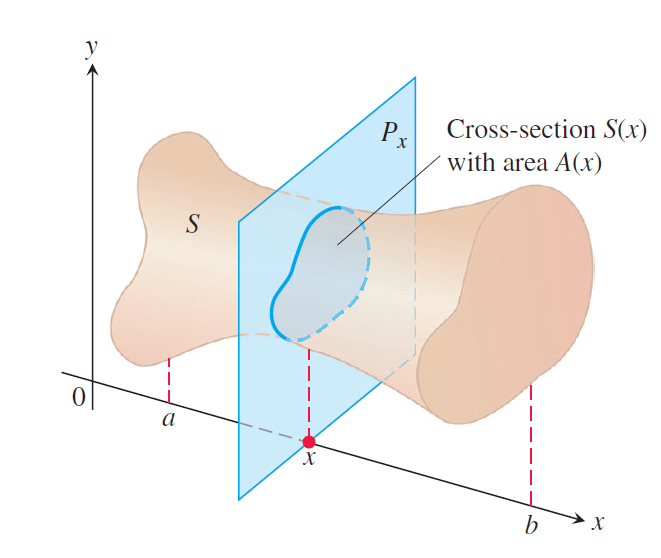
\includegraphics[width = 0.3\linewidth]{Images/cross-section.png}
     \caption{Cross-section Volume}
\end{figure}
\paragraph{Definition}
Let $S$ be a solid that lies between the planes $x = a$ and $x = b$. The volume $V$ of $S$ is defined by
\[
    V = \int_a^b A(x) dx
\]
provided that the cross-section area function $A(x)$ is integrable.
\paragraph{Example}
A curved wedge is cut from a circular cylinder of radius 3 by two
planes. One plane is perpendicular to the axis of the cylinder. The second plane crosses the
first plane at a 45° angle at the center of the cylinder. Find the volume of the wedge.
\begin{figure}[H]
    \centering
    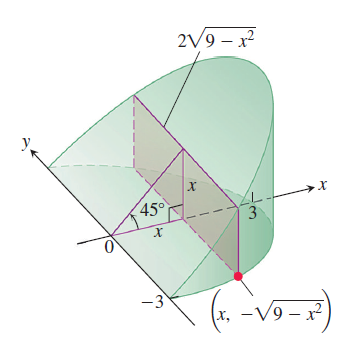
\includegraphics[width = 0.3\linewidth]{Images/cross-section ex1.png}
    \caption{Illustration of example 1}
\end{figure}

\paragraph{Answer}
The equation of the base circle is
\[
    x^2 + y^2 = 9
\]
So,
\[
    y = \pm \sqrt{9 - x^2}
\]
Since the angle of the cut its 45 degree, then the height of the cross-section is $x$
Then, the cross-section area is 
\[
    A(x) = 2x \sqrt{9 - x^2}
\]

\begin{align*} 
    V &= \int_0^3 2x \sqrt{9 - x^2}\: dx \\
    &\textrm{Let $u = 9-x^2$ then $du = - 2x dx$}\\
    &= \int_9^0 \sqrt{u}\: ( - du)\,\\
    &= \int_0^9 \sqrt{u}\: du \\
    &= \left[\frac{2}{3} u^{\frac{3}{2}}\right]^9_0 \\
    &= 18
\end{align*}
\subsection{Cavalieri's Principle}
Cavalieri's principle says that solid with equal altitudes and identical cross-sectional areas at each height have the same volume. This follows
from the definition of the volume, because the cross-sectional area $A(x)$ and the interval $[a, b]$ are the same for both solids.
\begin{figure}[H]
    \centering
    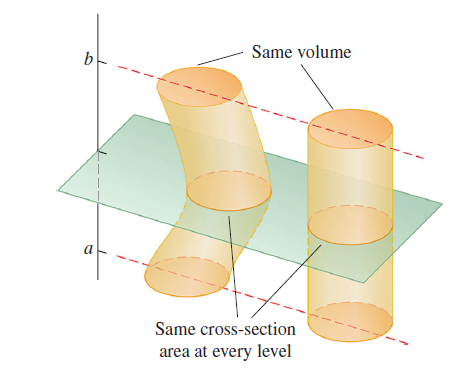
\includegraphics[width = 0.3\linewidth]{Images/cavalieri's principle.png}
    \caption{Cavalieri's Principle}
\end{figure}
\section{Solids of Revolution}
\subsection{The Disk Method}
\paragraph{Intuition}
If the solid $S$ is generated by rotating the region
\[
    \{(x, y): 0 \leq y \leq R(x), a \leq x \leq b\}
\]
around the x-axis, then the cross-sections of $S$ are discs with radii $R(x)$. Consequently 
\[
    A(x) = \pi R(x)^2
\]

\paragraph{Definition: Rotating around x-axis}
Volume by disks for rotation about x-axis with the radius of $R(x)$ is
\[
    V = \int_a^b A(x) dx = \int_a^b \pi [R(x)]^2 dx
\]

\begin{figure}[H]
     \centering
     \begin{subfigure}[b]{0.4\linewidth} 
          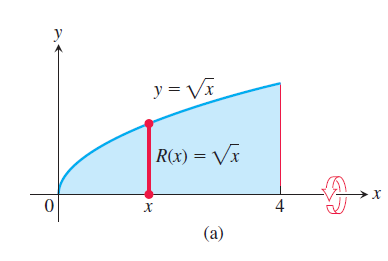
\includegraphics[width = 1\linewidth]{Images/solid of rev.png}
     \end{subfigure}
     \begin{subfigure}[b]{0.4\linewidth} 
        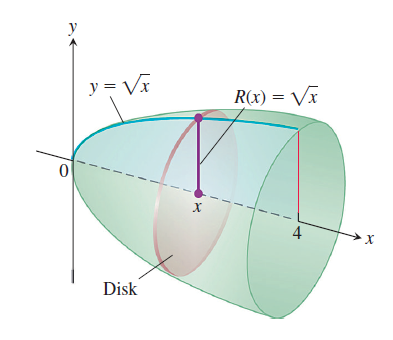
\includegraphics[width = 1\linewidth]{Images/solid of rev 2.png}
   \end{subfigure}
   \caption{Solid of rotation about x-axis}
\end{figure}
\paragraph{Definition: Rotating around y-axis}
Volume by disks for rotation about y-axis with the radius of $R(x)$ is
\[
    V = \int_a^b A(y) dy = \int_a^b \pi [R(y)]^2 dy
\]

\begin{figure}[H]
    \centering
    \begin{subfigure}[b]{0.3\linewidth} 
         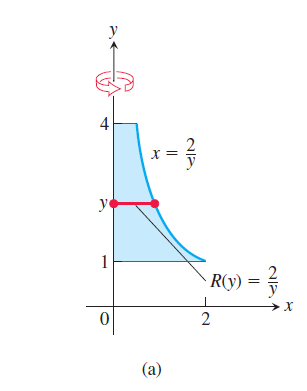
\includegraphics[width = 1\linewidth]{Images/solid of rev 3.png}
    \end{subfigure}
    \begin{subfigure}[b]{0.4\linewidth} 
       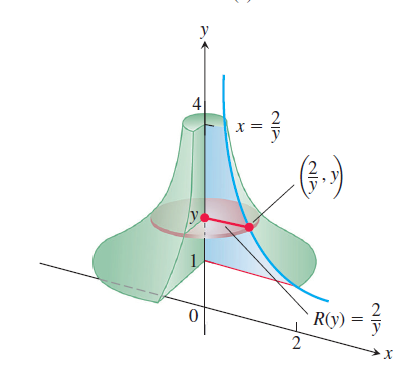
\includegraphics[width = 1\linewidth]{Images/solid of rev 4.png}
  \end{subfigure}
  \caption{Solid of rotation about y-axis}
\end{figure}

\paragraph{Example 1} What is the volume of $y = \sqrt{x}$ rotated about x-axis?
\begin{align*} 
    V &= \int_0^4 \pi (R(x))^2\: dx \\
    &= \int_0^4 \pi x\; dx \\
    &= \left[\frac{\pi}{2} x^2\right]^4_0 \\
    &= 8 \pi
\end{align*}

\paragraph{Example 2} The circle $x^2 + y^2 = a^2$ is rotated about x-axis to generate a sphere. Find its volume
\[
    R(x) = y = \sqrt{a^2 - x^2}
\]
\begin{align*} 
     V &= \int_{ - a}^{a} \pi (R(x))^2\: dx \\
     &= \int_{ - a}^a \pi (a^2 - x^2)\: dx \\
     &= 2\pi \int_{0}^a \pi (a^2 - x^2)\: dx \\
     &= 2\pi \left[a^2 x - \frac{1}{3}x^3 \right]_0^a \\
     &= \frac{4}{3}\pi a^3
\end{align*}

\subsection{The Washer Method}
\paragraph{Definition}
If the solid $S$ is generated by rotating the region 
\[
    \{(x, y) : 0 \leq r(x) \leq y \leq R(x), a \leq x \leq b \}
\]
around the x-axis, then similarly,
\[
    V = \int_a^b \pi(R(x)^2 - r(x)^2)\: dx
\]
for rotation around y-axis of
\[
    \{(x, y) : 0 \leq r(y) \leq x \leq R(y), a \leq y \leq b \}
\]
the volume is 
\[
    V = \int_a^b \pi(R(y)^2 - r(y)^2)\: dy
\]
\begin{figure}[H]
    \centering
    \begin{subfigure}[b]{0.4\linewidth} 
         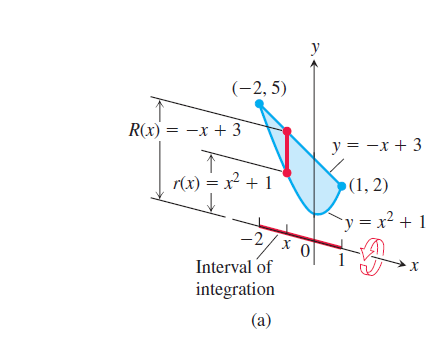
\includegraphics[width = 1\linewidth]{Images/washer method.png}
    \end{subfigure}
    \begin{subfigure}[b]{0.25\linewidth} 
       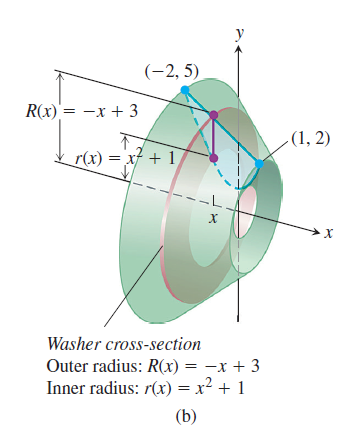
\includegraphics[width = 1\linewidth]{Images/washer method 2.png}
  \end{subfigure}
  \caption{The Washer Method}
\end{figure}

\paragraph{Example 1} The region bounded by the curve $y = x^2 + 1$ and the line $y = -x + 3$
is revolved about the x-axis to generate a solid. Find the volume of the solid.

First, find the limits of integration in the x-domain,
\[
    x^2 + 1= - x + 3
\]
We found $x = -2, y = 5$ and $x = 1, y = 2$.
\[
    V = \int_a^b \pi (R(x)^2 - r(x)^2)\, dx
\]
$R(x) = -x + 3$ and $r(x) = x^2 + 1$

\begin{align*} 
     V &= \pi \int_{ - 2}^{1} x^2 - 6x + 9 - (x^4 + 2x^2 + 1)\, dx \\
    &= \pi \int_{ - 2}^{1} - x^4 - x^2 - 6x + 8\: dx \\
    &= \pi \left[ - \frac{1}{5}x^5 - \frac{1}{3} x^3 - 3x^2 + 8x \right]^1_{ - 2} \\
    &= \frac{117}{5} \pi
\end{align*}

\paragraph{Example 2}
Find the volume of the solid obtained by rotating the region bounded by $y = 2\sqrt{x-1}$ and $y = x-1$ aboutthe line $x = -1$.

Since the rotation is about the line $x = -1$, we can create an equivalent revolution around the y-axis by shifting the plots
to the right by 1 unit, i.e. add 1 to each function.
\begin{align*} 
     &x = y + 1 \Rightarrow x = y + 2 \\
     &x = \frac{y^2}{4} + 1 \Rightarrow x = \frac{y^2}{4} + 2
\end{align*}

Then find the limits of integration in the y-domain where $x = y + 2$ and $x = \frac{y^2}{4} + 2$ intersect.
\begin{align*} 
     y + 2 &= \frac{y^2}{4} + 2\\
     0 &= y(y - 4) 
\end{align*}
$y = 0, x = 2$ or $y = 4, x = 6$

\begin{align*} 
    V &= \pi \int_{0}^4 (y + 2)^2 - (\frac{y^2}{4} + 2)^2 dy \\
    &= \pi \int_0^4 4y - \frac{y^4}{16} dy \\
    &= \pi \left[ 2y^2 - \frac{y^5}{80} \right]_0^4 \\
    &= \frac{96\pi}{5} 
\end{align*}


\paragraph{Example 3}
A region is bounded by $y = (x - 2)^2 + 1$ and $y = 5 - x$. Find the
volume of the solid generated by revolving the region around the y-axis.

Find the intersection points between the two functions. 
\[
    (x - 2)^2 + 1 = 5 - x
\]

\begin{figure}[H]
    \centering
    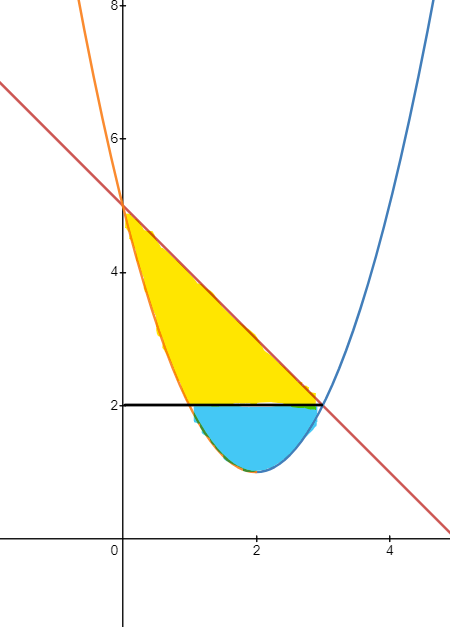
\includegraphics[width = 0.3\linewidth]{Images/ex3 solid of rev.png}
\end{figure}
Find the volume:
\begin{align*} 
    V &= \pi \int_2^5 (5 - y)^2 - ( - \sqrt{y - 1} + 2)^2 dy + \pi \int_1^2 (\sqrt{y - 1} + 2)^2 - ( - \sqrt{y - 1} + 2)^2 dy \\
    &= \frac{27\pi}{2} 
\end{align*}
\section{Cylindrical Shells}
\paragraph{Intuition}
Consider revolving the region in blue about the y-axis to generate a solid. Its volume can be computed by adding the volumes of 
all the "cylindrical shells".
\begin{figure}[H]
     \centering
     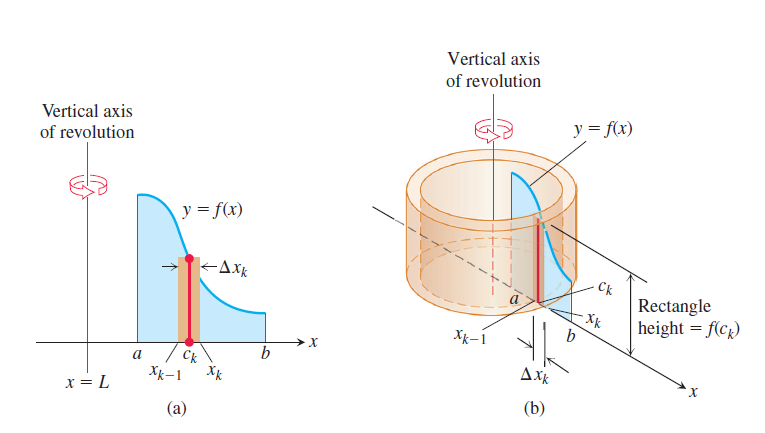
\includegraphics[width = 0.6\linewidth]{Images/cylindrical shell.png}
     \caption{Volume with cylindrical shells}
\end{figure}
Volume of a "thin cylindrical shell" or "thin annullus" is approximately the volume of cuboids of heigh $h(x)$ and the length $2\pi x$.
The height of cylindrical shell can be denoted as 
\[
    h(x) = f(x) - g(x)
\]
\begin{figure}[H]
     \centering
     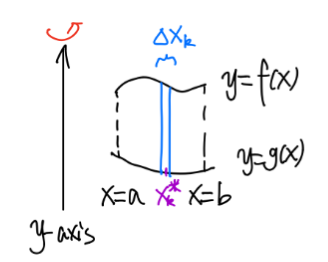
\includegraphics[width = 0.4\linewidth]{Images/cylindrical shell 2.png}
\end{figure}
The volume of the cylindrical shell at x is $V_k \approx 2\pi x_k^{*} h(x_k)^* \Delta x_k$.
Hence, the total volume 
\[
    V \approx \sum_{k = 1}^n 2\pi x_k^* h(x_k)^* \Delta x_k
\]

\paragraph{Definition}
Given the solid $S$ generated bu revolving the region
\[
    \{(x, y) : g(x) \leq y \leq f(x), a \leq x \leq b \}
\]
about y-axis, let $h(x) = f(x) - g(x)$ be the height of the region at $x$. Then 
the volume $V$ of $S$ can be computed by
\[
    V = \int_a^b 2 \pi x h(x)\: dx
\]

\paragraph{Example 1}
A region is bounded by $y = (x - 2)^2 + 1$ and $y = 5 - x$. Find the
volume of the solid generated by revolving the region around the y-axis.

\begin{align*} 
    V &= \int_0^3 2 \pi x (5 - x - (x - 2)^2 - 1) dx \\
    &= 2\pi \int_0^3 x(5 - x - (x^2 - 4x + 4) - 1) dx \\
    &= 2\pi \int_0^3 x( - x^2 + 3x) dx \\
    &= 2\pi \left[ - \frac{1}{4} x^4 + x^3 \right]_0^3 \\
    &= \frac{27\pi}{2} 
\end{align*}

\paragraph{Example 2}
Find the volume of the solid generated by revolving the region between $y = \sqrt{x}$ and $y = 0$ from 
$x = 0$ to $x = 1$ around the x-axis in two different ways.

(1) Using solid of revolution
\begin{align*} 
     V &= \pi \int_0^1 x dx \\
     &= \pi \left[ \frac{1}{2} x^2 \right]_0^1 \\
     &= \frac{\pi}{2}
\end{align*}

(2) Using cylindrical shells
\begin{align*} 
    V &= 2 \pi \int_0^1 y(1 - y^2) dy \\ 
    &= 2 \pi \int_0^1 y - y^3 dy \\
    &= 2 \pi \left[ \frac{1}{2} y^2 - \frac{1}{4} y^4 \right]_0^1 \\
    &= \frac{\pi}{2}
\end{align*}

\section{Arc Length}
\paragraph{Intuition}
Consider a curve given by a continuous function $y = f(x)$ defined on the interval $[a, b]$ and let 
$P$ be a partition of $[a, b]$.

If $y_k = f(x_k)$ and $\Delta y_k = y_k - y_{k-1}$, then the length of the curve between the points
$(x_{k-1}, y_{k-1})$ and $(x_k, y+k)$ is approximately 
\[
    L_k = \sqrt{(\Delta x_k)^2 + (\Delta y_k)^2} = \sqrt{1 + \left(\frac{\Delta y_k}{\Delta x_k}  \right)^2} \Delta x_k
\]
The definition of arc length is obtained by taking the limit of $\sum_{k = 1}^n L_k$ as $||P|| \to 0$

\begin{figure}[H]
     \centering
     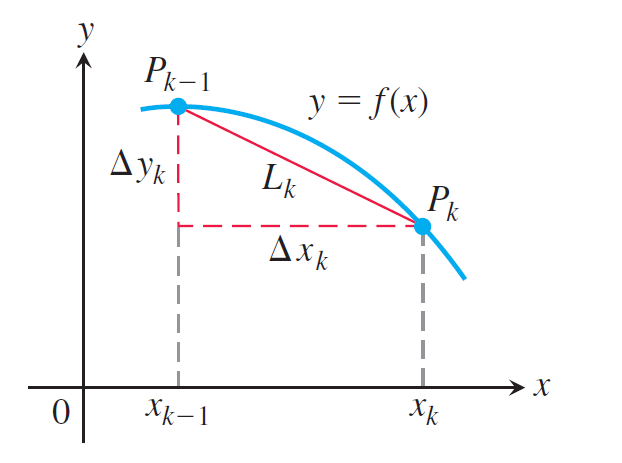
\includegraphics[width = 0.4\linewidth]{Images/arc length.png}
\end{figure}
\paragraph{Definition}
Let $f$ be a function such that $f'$ is continuous on $[a, b]$. The length/arc length $L$ of the curve $y = f(x)$ between the
points $(a, f(a))$ and $(b, f(b))$ is defined by
\[
    L = \int_a^b \sqrt{1 + \left(\frac{dy}{dx} \right)^2} dx = \int_a^b \sqrt{1 + (f'(x))^2} dx
\]

\paragraph{Example 1} Compute the length of the curve given by $y = x^{3/2}$, $0 \leq x \leq 3$

\[
    \frac{dy}{dx} = \frac{3}{2} x^{\frac{1}{2}}
\]

\begin{align*} 
    L &= \int_0^3 \sqrt{1 + \left( \frac{3}{2} x^{\frac{1}{2}} \right)}\:  dx \\
    &= \int_0^3 \sqrt{1 + \frac{9}{4}x}\: dx
\end{align*}

Let $u = 1 + 9/4 x$, $du/dx = 9/4, dx = 4/9 du$
\begin{align*} 
    L &= \int_1^{\frac{31}{4}} \sqrt{u} \frac{4}{9}\: du \\
    &= \frac{4}{9} \left[ \frac{2}{3} u^{\frac{3}{2}} \right]_1^{\frac{31}{4}} \\
    &= \frac{8}{27} \left( \left( \frac{31}{2} \right)^{\frac{3}{2}} - 1 \right)
\end{align*}

\paragraph{Note} If the curve is given by $x = g(y)$, $c \leq y \leq d$, and $g'$ is continuous, then 
the arc length is 
\[
    L = \int_c^d \sqrt{1 + \left(\frac{dx}{dy} \right)^2} dy = \int_c^d \sqrt{1 + (g'(y))^2} dy
\]
\section{Areas of Surfaces of Revolution}
\begin{figure}[H]
    \centering
    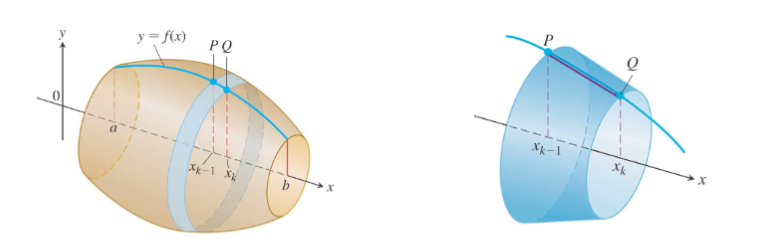
\includegraphics[width = 0.8\linewidth]{Images/solid surface.png}
    \caption{Cylindrical surface}
\end{figure}
\paragraph{Intuition}
We want to determine the area of a surface generated by revolving about the x-axis a curve $y = f(x)$, where $f$ is non-negative, for $x \in [a, b]$
Consider a cylindrical surface, generated by revolving a horizontal line around the x-axis.
\[
    A = 2\pi y \Delta x
\]
\begin{figure}[H]
     \centering
     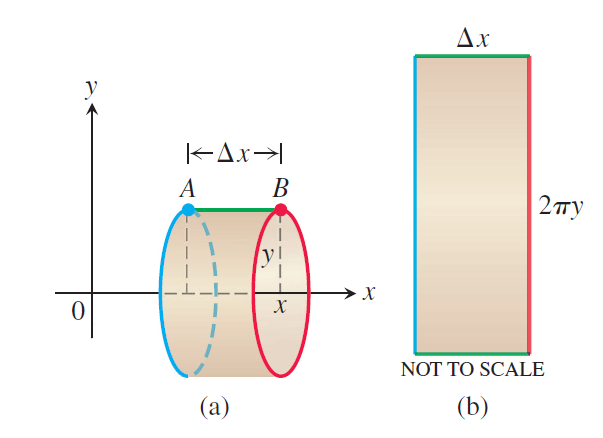
\includegraphics[width = 0.6\linewidth]{Images/cylindrical surface.png}
     \caption{Cylindrical surface}
\end{figure}
Consider a conical frustum generated bu revolving a straight line around x-axis.
\begin{align*} 
     A = 2 \pi y^* L \\
     y^* = \frac{y_1 + y_2}{2} \\
     A = \pi (y_1 + y_2) L 
\end{align*}
\begin{figure}[H]
    \centering
    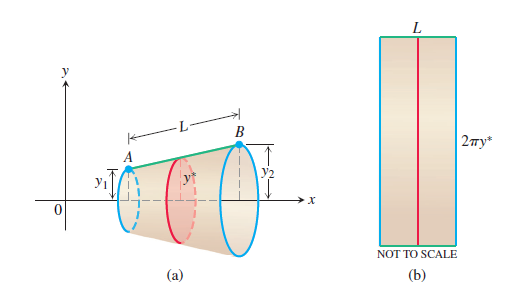
\includegraphics[width = 0.6\linewidth]{Images/conic fustrum.png}
    \caption{Conic Fustrum surface}
\end{figure}
For area of a surface of revolution about the x-axis in general, we make a partition $[a, b]$.
The $k$ portion of the curve has the length $\approx \sqrt{1 + \left(\frac{\Delta y_k}{\Delta x_k} \right)^2} \Delta x_k$
The area is approximately
\[
    A \approx \pi (f(x_{k - 1})) + f(x_k)) \sqrt{1 + \left(\frac{\Delta y_k}{\Delta x_k} \right)^2} \Delta x_k
\]

\paragraph{Definition}
If the function $f(x) \geq 0$ is continuously differentiable on $[a, b]$, the area of the surface generated by revolving the graph $y = f(x)$
about the x-axis is 
\[
    S = \int_a^b 2 \pi y \sqrt{1 + \left( \frac{dy}{dx} \right)^2}\: dx = \int_a^b 2 \pi f(x) \sqrt{1 + f'(x)^2}\: dx
\]
and if the function $g(y) \geq 0$ is continuously differentiable on $[c, d]$, the area of the surface generated by revolving the graph of $x = g(y)$ about y-axis is 
\[
    S = \int_c^d 2 \pi x \sqrt{1 + \left( \frac{dx}{dy} \right)^2}\: dy = \int_c^d 2 \pi g(y) \sqrt{1 + g'(y)^2}\: dy
\]

\paragraph{Example}
The curve $y = x^{1/3}$, $0 \leq x\leq 1$ is revolved about the y-axis to generate a surface. The area is?

$x = y^3$, $0 \leq y \leq 1$, $dx/dy = 3y^2$

\begin{align*} 
     S = \int_0^1 2 \pi y^3 \sqrt{1 + 9y^4}\: dy
\end{align*}
Let $u = 1 + 9y^4$, $du/dy = 36 y^3$
\begin{align*} 
     S &= 2 \pi \int_1^10 \sqrt{u} \frac{1}{36}\: du \\
     &= \frac{\pi}{18} \left[ \frac{2}{3} u^{\frac{3}{2}} \right]_1^10 \\
     &= \frac{\pi}{27}(10^{\frac{2}{3}} - 1)
\end{align*}

\section{Work}
\paragraph{Intuition}
If a constant force $F$ moves an object along a straight line for a distance $d$, then the work done by $F$ to the object is $W = Fd$
If a variable force $F$ moves an object the x-axis, and $F = F(x)$ depends on the position and $F$ is continuous on $[a, b]$, we make a partition $[a, b]$. Work 
done from $x_{k-1}$ to $x_k \approx F(x_k)\Delta x_k$. The total work then is approximately 
\[
    \sum_{k = 1}^n F(x_k) \Delta x_k
\]

\paragraph{Definition}
The work done by a variable force $F(x)$ in moving an object along the x-axis from $x = a$ and $x = b$ is 
\[
    W = \int_a^b F(x)\: dx
\]

\paragraph{Example 1} 
\textbf{Hooke's Law} states that the force required to stretch or compress a spring is directly proportional to its distance
$x$ away from the natural position of the spring
\[
    F(x) = k x
\]
What is the work required to compress a spring from its natural length of 30 cm to a length of 20 cm?
\begin{align*} 
     W = \int_0^0.1 F(x)\: dx &= \int_0^0.1 kx\: dx \\
     &= \left[ \frac{1}{2} k x^2\right]_0^0.1 \\
     &= 0.005 k J
\end{align*}

\paragraph{Example 2}
The conical tank is filled to within 2 m of the top with olive oil weighing 0.9 $g/cm^3$ or 8820 $N/m^3$. How much work does it take to pump the oil to the rim?
\begin{figure}[H]
     \centering
     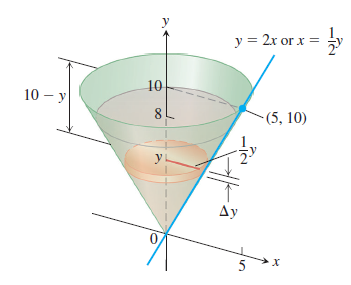
\includegraphics[width = 0.4\linewidth]{Images/work example.png}
     \caption{Illustration of the conical tank}
\end{figure}

\paragraph{Answer}
The typical volume of the slab has the volume
\[
    \Delta V = \pi \left(\frac{1}{2} y \right)^2 \Delta y = \frac{\pi}{4} y^2 \Delta y
\]

The force $F(y)$ is 
\[
    F(y) = 8820 \Delta V = \frac{8820 \pi}{4} y^2 \Delta y 
\]

Hence, the work needed is 
\[
    \Delta W = F(y) s = \frac{8820 \pi}{4} (10 - y) y^2 \Delta y 
\]

\begin{align*} 
     W &= \int_0^8 \frac{8820 \pi}{4} (10 - y) y^2 dy \\
    &= \frac{8820 \pi}{4} \int_0^8 10y^2 - y^3\: dy \\
    &= \frac{8820 \pi}{4} \left[ \frac{10y^3}{3} - \frac{y^4}{4} \right]_0^8\,\\
    &\approx 4.73 \times 10^6 J
\end{align*}


\section{Fluid Forces}
\paragraph{Pressure}
Pressure is the force that a fluid exerts on a surface divided by the surface's area.
\[
    p = \frac{F}{A} \textrm{\tab} \Rightarrow \textrm{\tab} p = \frac{dF}{dA}
\]

For a static liquid the pressure $p$ at depth $h$ is given by
\[
    p = wh
\]
where $w$ is the weight-density, or $\rho g$. 

For a container with a horizontal base, the total force applied by the fluid to the base is $F = pA = whA$
where $A$ is the base area.

\begin{figure}[H]
    \centering
    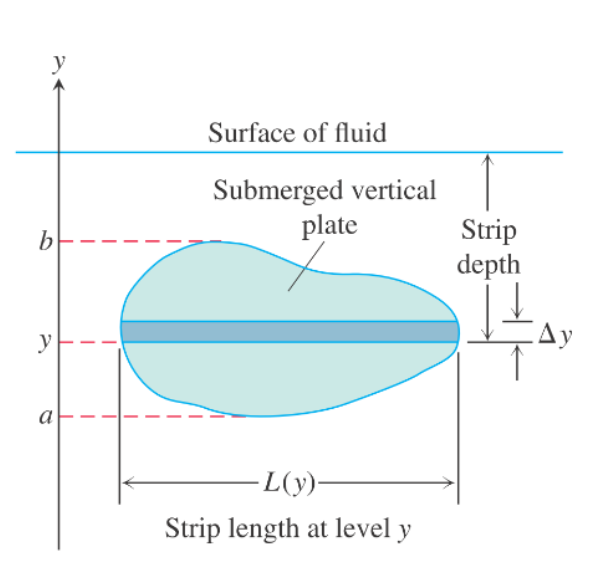
\includegraphics[width = 0.4\linewidth]{Images/fluid force.png}
    \caption{The force exerted by a fluid against one side of a thin horizontal strip}
\end{figure}
If a flat plate is submerged vertically, the pressure against it depends on the depth of the portion of the plate.
First, we divide the plate into horizontal thin slices $S_k$ with the width of $\Delta y_k$, depth of $h_k^*$, length of $L(y_k^*)$ and area 
of $L(y_k^*)\Delta y_k$. The force exerted on $S_k$ is 
\[
    F_k = whA \approx wh_k^* L(y^*_k) \Delta y_k
\]
Then the total force exerted on plate:
\[
    F \approx \sum_{k = 1}^n wh_k^* L(y_k^*) \Delta y_k
\]
The total force then is:
\[
    F = \int_a^b wh(y)L(y)\: dy
\]

\paragraph{Definition}
Suppose that a plate submerged vertically in the fluid of weight-density $w$ runs from 
$y = a$ to $y = b$ on the y-axis. Let $L(y)$ be the length of the horizontal strip measured from left to right along the surface of the plate
at level $y$ and $h(y)$ is the strip depth measured from the top of the fluid, then the force exerted by the fluid against one side of the plate is 
\[
    F = \int_a^b wh(y)L(y)\: dy
\]

\paragraph{Example}
A flat isosceles right-triangular plate with base 2m and height 1m is
submerged vertically, base up, 0.6 m below the surface of a swimming pool. Find the force
exerted by the water against one side of the plate.

\begin{figure}[H]
    \centering
    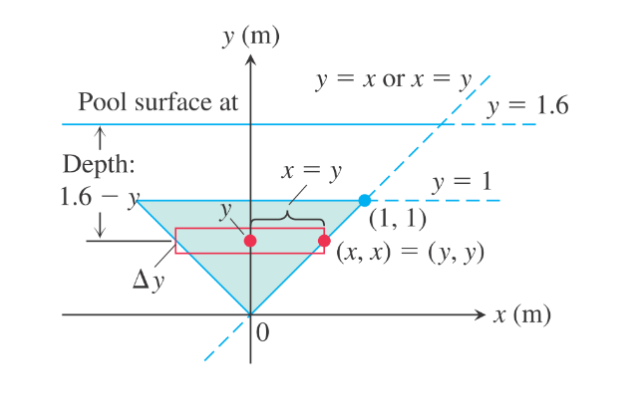
\includegraphics[width = 0.4\linewidth]{Images/fluid force ex.png}
\end{figure}

\paragraph{Answer}
\begin{align*} 
    F &= \int_a^b wh(y)L(y)\: dy \\
    &= \int_0^1 9800(1.6 - y)2y\, dy \\
    &= 19600 \int_0^1 (1.6y - y^2)\: dy \\
    &= 19600 \left[0.8y^2 - \frac{y^3}{3} \right]^1_0 \approx 9147 N
\end{align*}
\end{document}